\chapter{Poroelastic natural coatings}

\chapquote{Nature is the source of all true knowledge. She has her own logic, her own laws, she has no effect without cause nor invention without necessity}{}{Leonardo Da Vinci}


\section{Introduction to \textit{biomimetics}}

Usually when we are asked to imagine some fast-moving object as an airplane, a boat or a car, common sense leads us to think that its surface should be as smooth as possible.
However, if we look around, Nature seems not to agree with the previous statement.
In fact most of the surfaces in Nature are not at all smooth, they almost always present more or less regular arrangements of discontinuities at various length scales.
Since Nature had a very long time-span to optimize this kind of surfaces we can suppose that they are the best possible options.
One should pinpoint that the non-smoothness of these surfaces can be connected to some other biological functions rather than to pure fluid dynamics performance, and of course this can be the case.

An example of natural surface is the shark skin, in figure \ref{fig:shark} where a segment of the skin is depicted, as it appears under the microscope.

\begin{figure}[h]
	\centering
	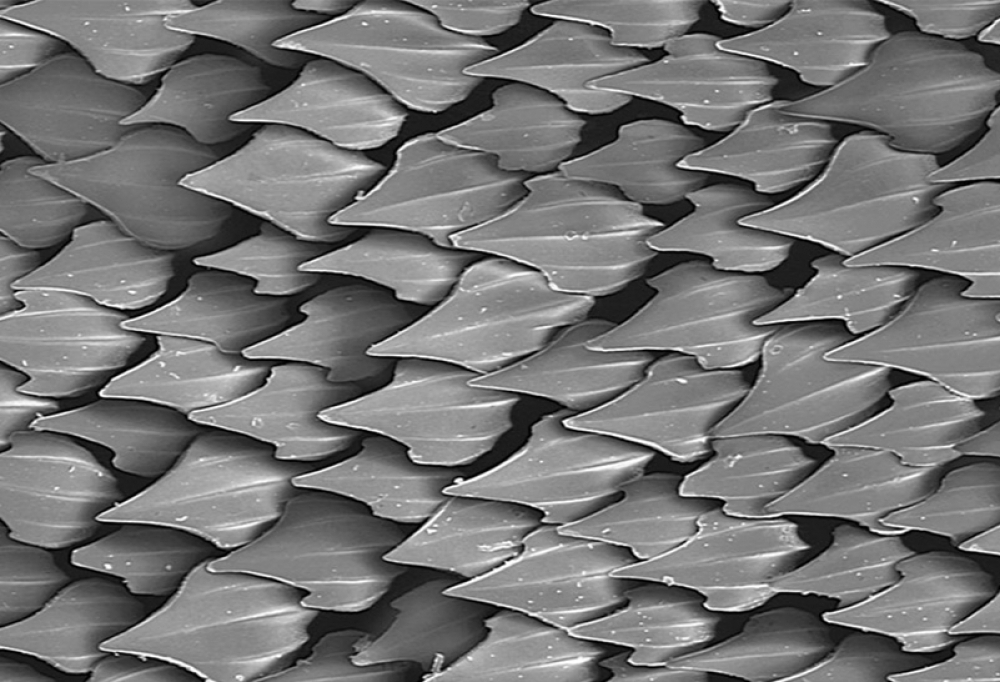
\includegraphics[width=0.6\linewidth]{chapter_1/shark}
	\caption{Microscope enlarged picture of the shark skin.}
	\label{fig:shark}
\end{figure}

The enlargement shows that the surface is made up by a series of overlapped denticles, and experiments show that they can move and interact with the flow. This interaction is supposed to reduce the shark drag when swimming.

The shark "technology" has somehow been applied by Speedo$^{\circledR}$. This company has designed famous swimming suits with a surface that mimics the shark skin. Numerous swimmers have broken several world records wearing this swimming suits.
This controversial swimmers' performance was due to the fact that the swimsuit compressed the body giving the swimmer a more streamlined shape.
Even thought the company has publicized their product as if it were a synthetic shark skin, \citet{Oeffner785} have shown that the texture of such swimming suits is somehow different from the shark dermal structure.
In their work the authors have performed swimming experiment of a flat plate with different coatings and they did not found significant speed enhancement with a swimsuit-like surface, but the measurements with real shark skin on the contrary have demonstrated an appreciable improvement of performances.

Poroelastic surfaces find also applications in aeroacoustics; owls are well known for their particularly silent flight, especially in the high frequency spectrum.
This characteristic is crucial for the owl in order to capture its preys.
Obviously it has inspired the scientific community to study their feathers' configuration and shape.

\begin{figure}[h]
	\centering
	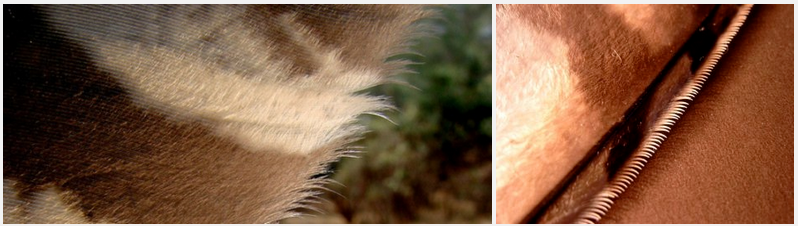
\includegraphics[width=0.8\linewidth]{chapter_1/howl}
	\caption{Feathers on owl's wing. Left: trailing edge. Right: leading edge. The differences in shape and mechanical properties, such as rigidity, between the leading and the trailing edges, is a consequence of the different flow regimes in the wing.}
	\label{fig:owl}
\end{figure}
 
Several authors have shown promising results in characterizing the acoustic properties of the owl's skin and their physical mechanisms.
In particular \citet{lilley1998} presented three main characteristics of the owl, which can suppress its airborne noise: i) the comb shaped feathers in the leading edge, ii) the fringe at the trailing edge, iii) the presence of numerous "filaments" in the bottom surface of wings and legs.

Another example is described in the work by \citet{jaworski2013aerodynamic} who studied the acoustic scattering problem of a poroelastic half-plane encountering an incident plane wave.
This configuration, a simplified owl's wing, explains how the properties of this surface can suppress the noise.
They concluded that the combined effects of elasticity and porosity can produce a weaker noise amplification.

Recent computational simulations performed by \citet{rao2017owl} confirm that the leading edge shape of the feathers truly suppresses noise and enhances the lift generation.

Another example of bioinspired aerodynamic surfaces is the butterflies' wing.
In figure \ref{fig:butterfly} the surface of a "Peacock butterfly" is enlarged in order to show the multiple scales involved. The wing structure present firstly a series of overlapped scales similar to the shark, but if we look closely it can be observed that each scale has a complicate permeable structure.

\begin{figure}[h]
	\centering
	\begin{subfigure}[b]{0.3\textwidth}
		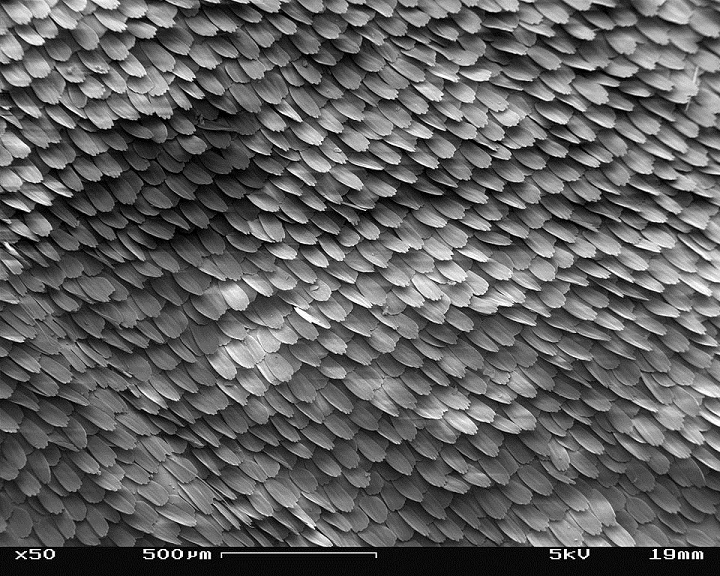
\includegraphics[width=\textwidth]{chapter_1/butterfly}
		\caption{Magnification 50x}
		\label{fig:b50}
	\end{subfigure}
	~ %add desired spacing between images, e. g. ~, \quad, \qquad, \hfill etc. 
	%(or a blank line to force the subfigure onto a new line)
	\begin{subfigure}[b]{0.3\textwidth}
		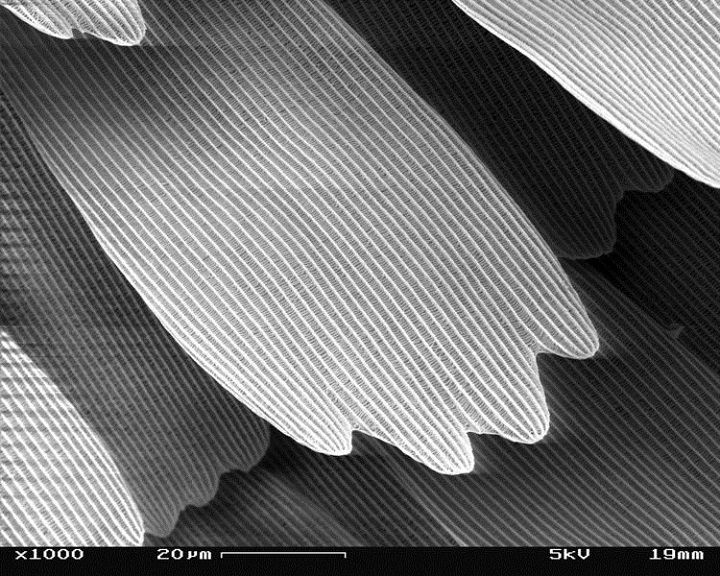
\includegraphics[width=\textwidth]{chapter_1/butterfly2}
		\caption{Magnification 1000x}
		\label{fig:b1000}
	\end{subfigure}
	\begin{subfigure}[b]{0.3\textwidth}
		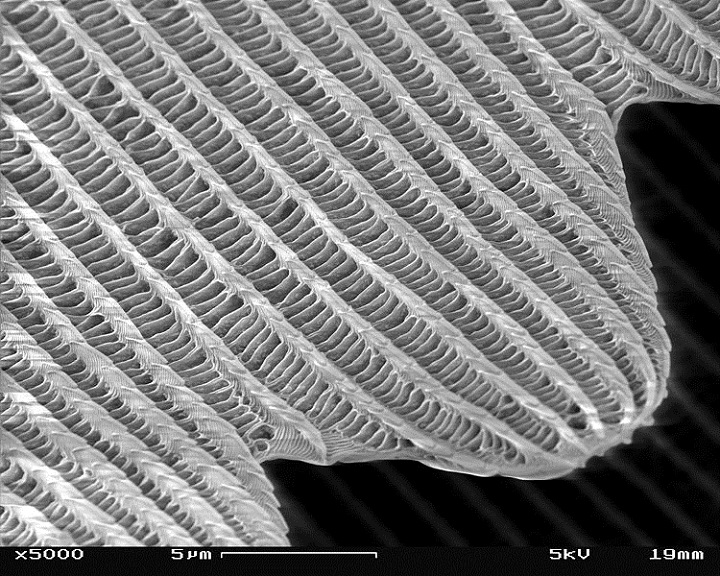
\includegraphics[width=\textwidth]{chapter_1/butterfly3}
		\caption{Magnification 5000x}
		\label{fig:b5000}
	\end{subfigure}
	\caption{Particular of a Peacock butterfly wing, taken with a Scanning Electron Microscope. Images from wikimedia.org}
	\label{fig:butterfly}
\end{figure}

\citet{slegers2017beneficial} have studied the effect of such porous structure on the flight performance of butterflies.
Using cameras to measure the kinematics of their flight, they can measure their efficiency to "climb" (i.e. generate lift) and the stroke amplitude and frequency.
The authors conclude that the porous structure of their wing gives a boost in climbing efficiency of $30\%$. This result clearly stresses out the importance of the poroelastic coating of the wings. 
Even though the butterfly flight aerodynamic is extremely complex, it is clear that the peculiar structure of the wing's surface is critical for their aerodynamic performances, as also \citet{srygley2002unconventional} had confirmed.

The last example concerns super-hydrophobic surfaces. These surfaces, such as that of the lotus leaf, are water repellent, i.e. water can slide over them with less resistance, because of the surface's low wettability.
This behavior is caused by the microscopic structure which forms the surface (see figure \ref{fig:lotus}). In reality the roughness elements are arranged in a quasi-regular way, in order to be able to capture air pockets that rest within the "valleys". These air inclusions provoke an effective slip at the air-liquid interface that causes skin friction reduction. They also change the contact angle of the droplets. The work of \citet{bottaro2003effect} summarizes some of the above super-hydrofobicity aspect and their applications.

\begin{figure}[t]
	\centering
	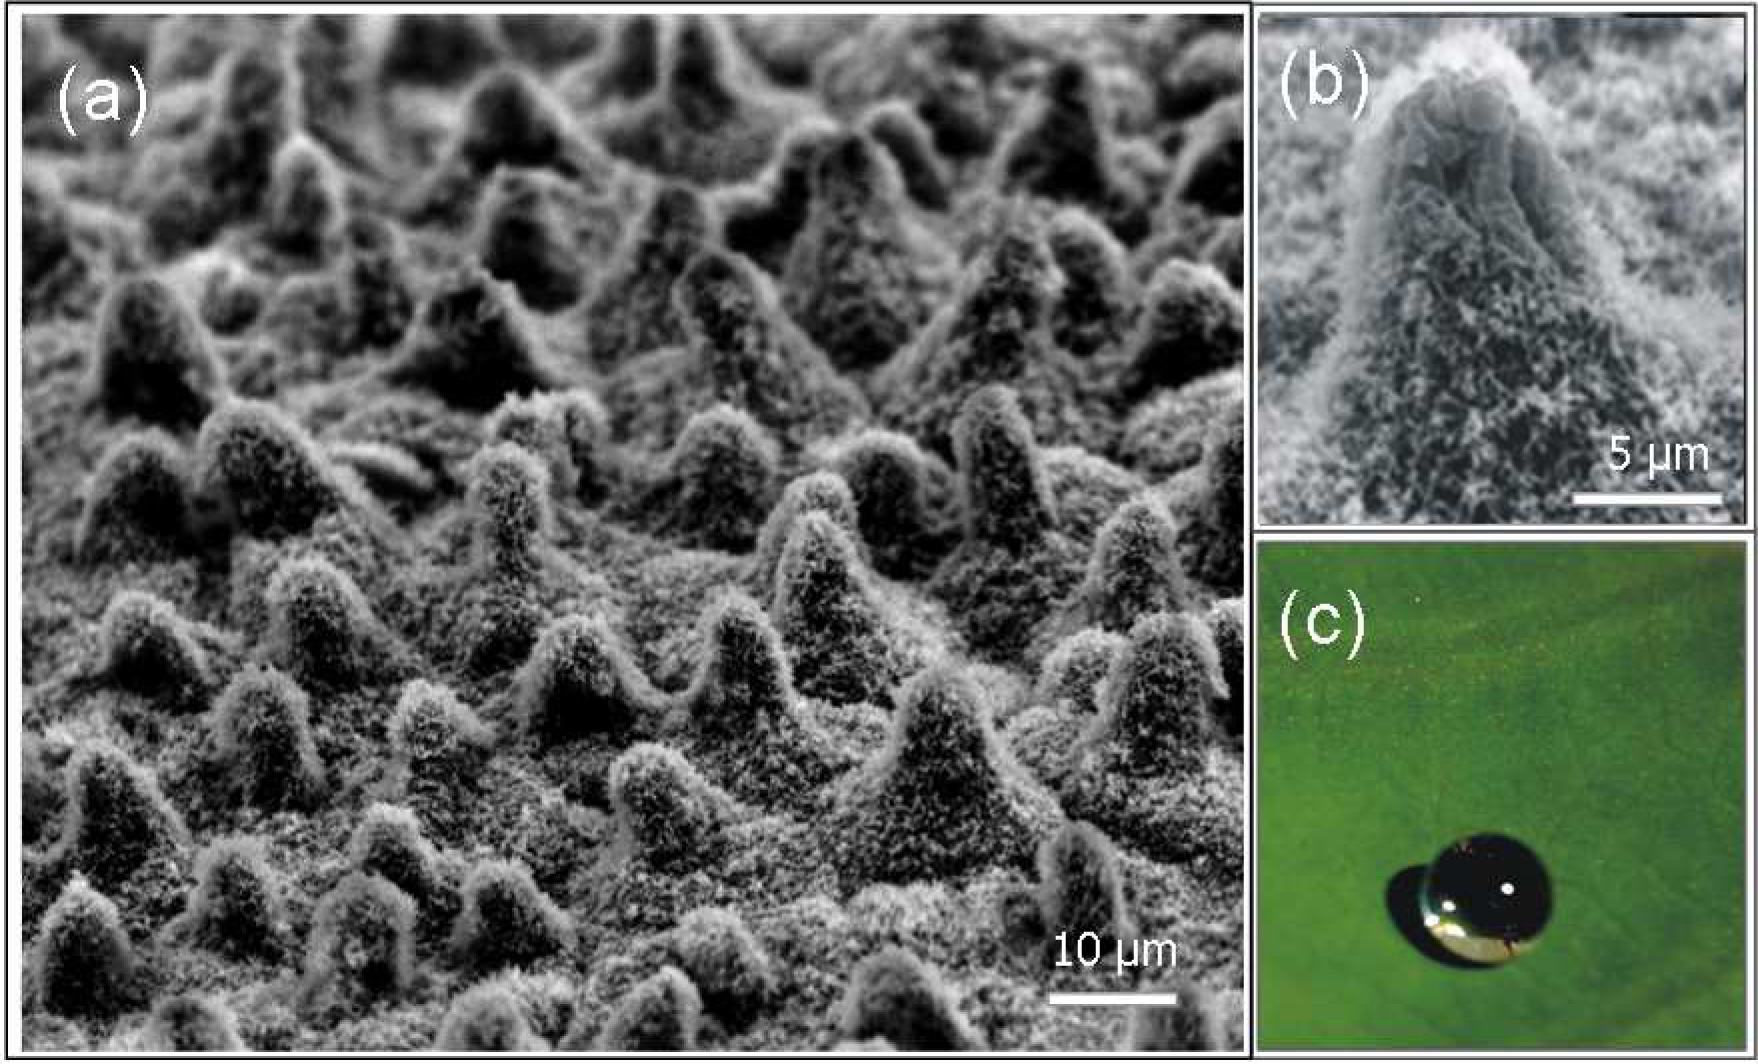
\includegraphics[width=0.6\linewidth]{chapter_1/lotus}
	\caption{(a) Scanning electron microscopy (SEM) image showing the structure of a lotus leaf, (b) higher order of magnification on the single protuberance forming the surface and (c) water drop with high contact angle, attaining an almost spherical shape. Images from \citet{stratakis2009laser}.}
	\label{fig:lotus}
\end{figure}

Interested readers can find more examples of biomimetics and broaden the above key aspect in \citet{bhushan2016biomimetics} and \citet{tropea2012nature}.

\section{Riblets and shark-skin surfaces}
We have shown that natural surfaces can be an inspiration to find strategies in solving many problems concerning aerodynamics. In the following we especially focus on drag reduction.

It is known that the total drag contribution can be separated into different components and the classical decomposition is between viscous drag (sometimes referred to as skin friction) and pressure drag.

\begin{equation}
 \int_{A_{\sigma}}  [ \underbrace{\left({p} \mathbf{I} \right) \cdot  \mathbf{n}_{\sigma} }_\text{pressure drag}  +  \underbrace{\boldsymbol{\tau}}_\text{viscous drag} ] \; dA,
 \label{eq:force}
\end{equation}

\noindent where the shear stress $\tau$, for incompressible flow, is defined as:
$$
\boldsymbol{\tau} = \mu \left( \nabla \mathbf{v} +  \nabla^T \mathbf{v} \right) \cdot  \mathbf{n}_{\sigma}
$$

\noindent In \eqref{eq:force} $A_{\sigma}$ is the solid interface of some body where a no-slip condition is usually applied and $ \mathbf{n}_{\sigma}$ is its outward normal unit vector.

\noindent The shear stress for incompressible flow in the turbulent case is often defined as:
\begin{equation}
\boldsymbol{\tau_t} =  (\mu + \mu_t)\left[ \nabla \mathbf{\overline{v}} +  \nabla^T  \mathbf{\overline{v}} \right] \cdot  \mathbf{n}_{\sigma}
\end{equation}
where $\mu_t$ is the turbulent viscosity and $\mathbf{\overline{v}}$ is the temporal average velocity.
This section is about the existing ways to reduce the viscous part of the drag working only on the surface texture.

\subsection{Riblets}
Most of the industrial applications involve turbulent flows, and as a results there is a lot of research that aims to reduce skin friction in this regime.
Table 6.3.1 in the book of \citet{mclean2012understanding} includes a wide list of techniques already been proposed on the problem.
As the same author pinpoints, the most effective and, probably the most practicable solution, is the surface texture known as riblets.
Riblets are alternating ridges aligned in the streamwise flow direction and regularly arranged, as figure \ref{fig:riblets1} shows.
These surfaces are capable to align the turbulent flow along the mean flow direction, smoothing the fluctuations of the crossflow in the viscous sublayer.
The turbulent momentum transfer is reduced as a consequence of reducing these fluctuations close to the surface. In the same manner the surface experiences a lower skin friction.

\begin{figure}[h]
	\centering
	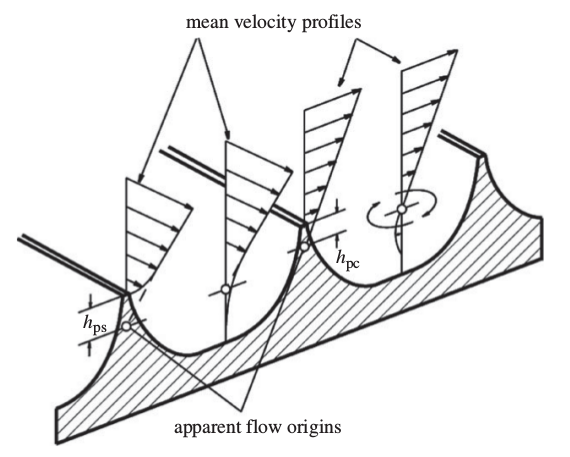
\includegraphics[width=0.7\linewidth]{chapter_1/riblets3}
	\caption{Schematics of the  \textit{protrusion height} concept. The mean velocity profiles for the stream-wise and crossflow velocities are shown. In presence of a ridge it is possible to extrapolate the point of zero velocity from the velocity gradient outside the riblet; finding respectively, the \textit{streamwise protrusion height} $h_{ps}$ and the \textit{cross-flow protrusion height} $h_{pc}$. Image from \citet{bechert1997experiments}.}
	\label{fig:riblets1}
\end{figure}

The viscous drag reduction correlates well with the spacing between the ridges expressed in wall units, $ s^+ $. The typical shape of the $\Delta \tau/\tau_0 \; - \; s^+$ relation is depicted in figure \ref{fig:riblets_perf}, where the vertical axis shows the drag reduction against $s^+$.
This general shape of the curve, in which the skin friction decreases in a certain range of spacing and then increases as the ridge spacing  increases, is caused by a competition between the capacity of riblets to obstruct lateral fluid flow and the increase of penetration of high speed vortices inside this manufactured wall irregularity.

\begin{figure}[h]
	\centering
	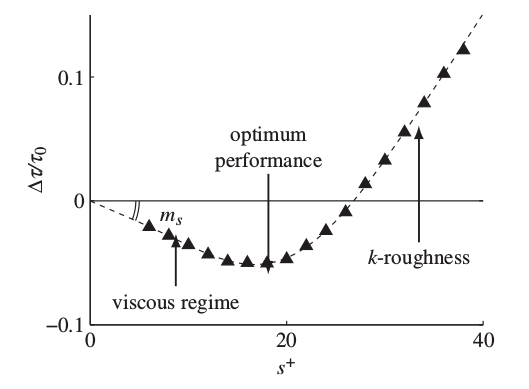
\includegraphics[width=0.5\linewidth]{chapter_1/riblets_performance}
	\caption{Example of drag reduction relation to the ridge spacing. The maximum performance is normally around $ s^+ = 15 $, the picture shows also that when the riblet are really tightely spaced the laminar case is retrieved. On the contrary when the riblets are far away from one another their performance is comparable to the  rough plate case. $\tau_{0}$ is the wall stress in the case of a smooth flat plate. Image from \citet{jimenez2001turbulent}. }
	\label{fig:riblets_perf}
\end{figure}

This last physical explanation of the riblets' performances is presented in the schematics \ref{fig:riblets_schem}, where the gray areas show high skin-friction regions caused by the downwash motion generated by the near-wall vortices.
It is clear that, when the riblets are too large, the vortices can penetrate inside the groove and increase the skin friction, due to a larger area exposed to the local velocity.
On the contrary, when the riblets are smaller, the high speed vortex only hits the tip of the ridges, so that, only a small local area of the surface experiences high-shear stresses.

\begin{figure}[h]
	\centering
	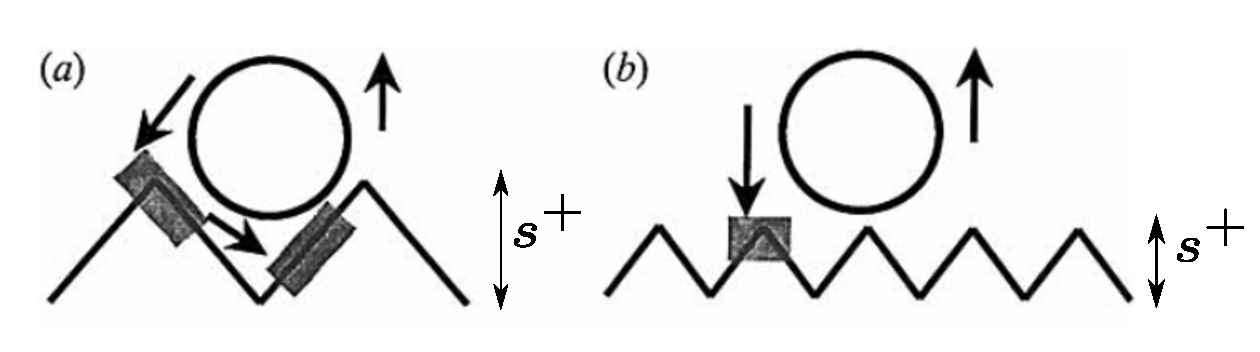
\includegraphics[width=0.7\linewidth]{chapter_1/riblets1}
	\caption{Two different sizes of riblets are shown when interacting with a sublayer vortex. In gray it is represented the area where friction is important. Clearly when both sizes are comparable the surface experience a larger friction and the performance is lowered. Image from \citet{choi1993direct}.}
	\label{fig:riblets_schem}
\end{figure}

The slope $m_s$ of the curve in figure \ref{fig:riblets_perf} can be predicted by linear stability theory (either in laminar and turbulent cases changing the definition of base flow) or by means of empirical correlations(see, e.g., \citet{garcia2011hydrodynamic}).

Computing the performance of such surfaces can be expensive, since the most reliable quantitative theory for such problems consist of direct numerical simulations (DNS) or experiments.
However there is one theory, besides the already cited expensive ones, that uses the concept of \textit{protrusion height}, shown in figure \ref{fig:riblets1}, to correlate the shape of these protrusions to the drag reduction (cf. \citet{luchini1991resistance}).
In this way the \textit{protrusion height} is defined as the vertical distance between the riblet top ridge and the point of zero velocity, extrapolated from the constant velocity gradient outside above the protrusions.
It appears that the difference of protrusion heights ($h_{ps} - h_{pc}$) correlates very well with the drag reduction. The two quantities can be computed with a simple Stokes problem over the local geometry of the grooves.
%The last result has been analyzed by \citet{segura2017permeable} that propose an empirical law for the drag reduction, relating the previous protrusion heights with the permeability expressed in wall units:
%
%\begin{equation}
%-\Delta \tau/\tau_0 = DR \approx 0.04\left( \sqrt{{K_s}^+} - \sqrt{{K_c}^+} \right),
%\label{eq:max_dr}
%\end{equation}
%
%where ${K^+}_s$ and ${K^+}_c$ are the streamwise and crossflow permeability tensor components.
%This law establishes a relation that help to estimate the drag reduction from a given geometry of the wall. The permeability tensor can be computed within the porous media homogenization approach as chapter \ref{ch:vans} explains.

Another important characteristic of riblets is that they are robust in off-design conditions, such as in presence of yaw (misalignment between flow and riblets ridges) and tip ridges erosion (\citet{garcia2011drag}).

Besides some very specific application such as sailing competitions (the hulls of the USA challengers in the America’s Cup 1987 and 2010), the massive use of this technology is still in question.
Producing such surfaces in a larger area, like the roof of a car or the wing of an airplane, can be an issue for a routine use, because riblets size needs to be very small to be effective. The riblets need also to be cleaned after each use otherwise some residue (like insect or vegetation) can modify the roughness of the surface and reduce their effectiveness.

Anyhow, riblets-like surfaces have been observed in Nature for many years, for example \citet{Martin2016riblets} found that skimmer birds (Rynchops) have riblets like grooves in their beak, since they fly with it under the water surface to catch fishes.
However, as already introduced, the most clear example of such natural surfaces is represented by the shark skin.

\subsection{Shark skin}
In their review, \citet{dean2010shark} present the status of the shape optimization that has been done on the riblets trying to mimic the typical sawtooth shape seen on shark skin, showing that improvements of such geometries over the classical ones has yet to be achieved.
Shape optimization on riblets geometry has been studied by \citet{bechert1997experiments}, showing that just few percents can be gained compared to the base line geometry.

There are, actually, some controversial results in the literature stating that surfaces, with actual shark skin replica, can indeed increase drag.
\citet{boomsma2016direct} performed some simulations on actual shark skin denticles using the immersed boundary method. These authors simulated various arrangements of the denticles and they found that, in some configurations, the actual drag increases up to $40\%$. This can be a clue that the shark skin does not work with the same mechanism as riblets do.

Experiments on such geometries are available in the literature (\citet{bechert1997natural}).
The authors built a synthetic surface, made by artificial shark denticles fixed on top of springs. They have shown that, even with the introduction of surface elasticity, the actual drag was increased.
However, they pinpointed that the actual shark flow regime was not steady in the experiments performed, and they speculated that the excellent swimming performance of the shark comes from the separation control that flexible denticles can operate during the periodic oscillating flow that the swimming generates.

In addition an experiment using DPIV on a NACA profile covered with actual skin samples of "Isurus oxyrinchus" mako shark, has been performed by \citet{lang2014SharkControl}, confirming that the flexibility of sharks denticles provides the passive flow control needed to avoid early separation.
In fact, the experiments have proven that for angles of attack larger than $15^{\circ}$ the flow reversal was almost completely avoided.
The same authors noted that different geometries of the denticles can be found in various parts of the shark body, and these differences can be important since flow conditions can change from the head to the tail.
\citet{motta2012Shark} performed a detailed collection of flexibility and scale measurement of different shark species that can be valuable for future studies.

Again, swimming experiments from \citet{Oeffner785}, who used a flat plate covered with real shark skin, confirmed the previous flow control mechanism. They had also made some conjectures about possible thrust enhancing, controlled by the same denticles, that can move away the leading edge vortex.

Also \citet{itoh2006turbulent} showed that movable rugosities can outperform riblets. They measured the drag reduction of a seal fur (that present fibrous movable surface) against a riblet surface in an experimental channel. Their results are show in figure \ref{fig:seal} in which it is visible that seal fur can outperform  rigid riblet performance by $5\%$ in a certain span of Reynolds numbers.

\begin{figure}[h]
\centering
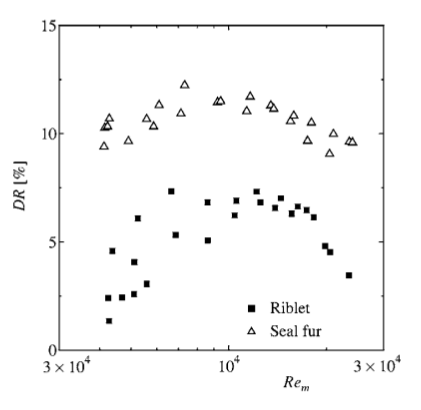
\includegraphics[width=0.5\linewidth]{chapter_1/seal}
\caption{Performance comparison between a riblet surface against a seal fur. The drag reduction has been computed as: $DR \% = \dfrac{ \Delta \tau}{\tau_{0}} \%$. Image from \citet{itoh2006turbulent}.}
\label{fig:seal}
\end{figure}


Compliant surfaces can, in reality, move accordingly to the surface pressure gradients along the boundary layer and so respond to the pressure fluctuations over the surface itself.
This mechanism is already known to be beneficial in delaying the transition to turbulence and many authors have presented theoretical and experimental evidence on the effectiveness of this solution (\citet{carpenter1990status}, \citet{bushnell1977effect}).

In conclusion, we have seen that, in order to reduce turbulent skin-friction drag, riblets and natural surfaces use various mechanisms such as: sublayer vortices interaction, compliance and separation control. Such solutions have proven to be effective in various cases mostly related to the viscous component of the drag.
In the next section we introduce another class of solutions that try to act mostly on the pressure component.


\section{Permeable surfaces}
As permeable surfaces we indicate permeable coatings that usually have a significant thickness; in contrast to riblets, in which the vertical extension outside the wall is limited.
In this case the flow can penetrate deep into the porous surface and generate complex interaction mechanisms.
The next sections presents an overview of the most notable applications of such permeable surfaces.

\subsection{Bluff bodies}

There is some experimental evidence that, in the laminar regime, generation of some \textit{slip velocity} at the interface between the permeable surface and a fluid, can decrease the skin friction (\citet{beaver}).
However, in the turbulent case it seems that the instabilities developing at the interface can cause a drag increase up to $40\%$ (\citet{jimenez2001turbulent}; \citet{breugem2006influence}); this instability mechanism is further explained in section \ref{sec:stability}.
It is important to observe that the permeable surfaces cited in the above references are all rigid.

The pressure contribution to the drag is usually the most significant one in bluff bodies applications, and even in highly streamlined body it is around $10\%$ of the total drag.
Researchers have tried to find a way to modify the pressure distribution around a bluff body to reduce the associated resistance, and also to damp the force oscillations on the body (drag and/or lift).

The pressure drag on a bluff body depends mostly on the difference between the low pressure on the rear part of the body, where there is usually a separated flow region, and the high pressure in the forward part.
This idea is sketched in figure \ref{fig:pressure_dist} where two different pressure distributions are shown; the black one represents the classical solid body, and the green one is the one with a porous layer at the back of the body.

\begin{figure}[h]
	\centering
	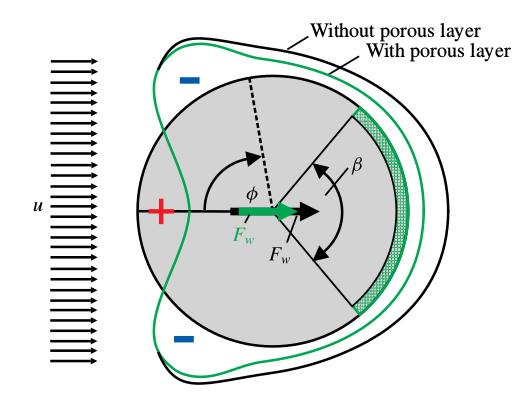
\includegraphics[width=0.4\linewidth]{chapter_1/pressure_dist}
	\caption{Diagram showing an example of angular pressure distribution around a cylinder for viscous flow. The black line is the case of a solid body, the green one is the modified pressure when a porous layer is present on the rear. Image from \citet{klausmann2017drag}.}
	\label{fig:pressure_dist}
\end{figure}

The favorable increase of pressure in the rear point is due to the low speed laminar flow in the porous media that is ejected in the back region where separation takes place.
Even in very high speed turbulent flows, the fluid inside the permeable surface exhibits a very high energy loss due to the strong dissipation that the medium provides, resulting in a low speed flow ejected downstream of the body.

The permeable interface, producing a slip velocity, can modify the boundary layer that develops above it producing less shear and vorticity, modifying also the stability characteristics of the flow.
The instability around a cylinder is due to the shear layer that forms in the top part of the body, when the flow starts to decelerate.
This shear layer exhibits a Kelvin-Helmholtz-type instability that develops in the classical Von-Karman wake.

These two hypothetical mechanisms has been tested using numerical simulations by several authors: \citet{bruneau2004passive} \cite{bruneau2008numerical}, \citet{bhattacharyya2011reduction}, \citet{naito2012numerical} and \citet{mimeau2017passive}.
These works studied the flow around some classical two dimensional bluff bodies (cylinder, square cylinder, Ahmed body section, 3D hemisphere) with the addition of a porous layer.

These works show some very promising results, like: decrease of enstropy, lower oscillations in lift, drag reduction, regularization of the wake and lower pressure gradients, even if the porous medium was rigid in the case treated.
An example of turbulent flow field downstream to a square cylinder is shown in figure \ref{fig:porous_cylinder}; the picture demonstrated how the porous layer strongly regularizes the wake.

\begin{figure}[h]
	\centering
	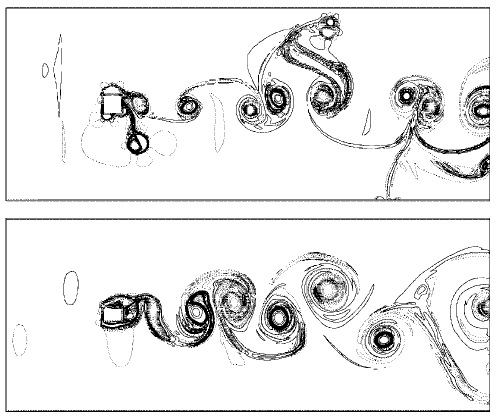
\includegraphics[width=0.7\linewidth]{chapter_1/cylinder_porous}
	\caption{Square cylinder vorticity contour for $Re=30000$. Top: solid case. Bottom: porous case with layer extension $h/D=10\%$.}
	\label{fig:porous_cylinder}
\end{figure}


The simulations performed by the authors above indicate that porous medium parameters, like the medium porosity or its vertical extension above the solid wall, have important effects on the quantities listed above.
The variety of these results seems to indicate (at least qualitatively) that increasing the porous medium extension beyond a certain limit is not beneficial, and they also show that the porosity of the medium should not be excessive in order to be effective (high/medium porosities are the best).

However the above cited works should be taken with some care; only few cases are three-dimensional, they all use a modeling approach for the porous medium based on a simplified version of the VANS (Volume Average Navier-Stokes equations, see section \ref{sec:vans}), without performing any validation of the method.
Sometimes they also use the equations outside their field of validity (there are discussions in the scientific community about using the previous version of the VANS equations for highly turbulent flows).

The lack of validation reflects the fact that reliable experiments of such porous coatings are almost non existent in the literature.
There is also some confusion in the community on how to compute forces on such bodies surrounded by a porous coating. These differences led some authors ( \citet{naito2012numerical}) to over-estimate the forces and their predictions are not aligned with the literature.
\citet{caltagirone1994interaction} argued on theoretical bases that the approach used by \citet{bruneau2004passive} is the correct one for that specific version of the VANS used by all the previous authors. 

%\begin{equation}
%	\mathbf{F} = \int_{\Omega_p} \varepsilon \mub \mathbf{K}^{-1} \vbmi \; dV
%\end{equation}
%where $\mub$ is the dynamic viscosity of the fluid, $\varepsilon$ is the porosity, $\mathbf{K}$ is the permeability of the porous medium, $\vbmi$ the intrinsic averaged velocity and $\Omega_p$ the porous domain.
 
The approach of \citet{favier2009passive} differentiates itself from the previous approaches that use the VANS equations. In fact the authors used a numerical method that includes the dynamics of a moving porous medium made of fibers at the back of a cylinder.
Their results in a laminar flow case agree with the prediction of a wake stabilization and show some more realistic values of drag reduction, about $15\%$.
However the difficulties in this approach lie in the medium dynamics, it introduce many mechanical parameters that are not easily identifiable for natural surfaces.

A similar model has been used by \citet{venkataraman2012numerical}, in which they applied a movable porous coating in the suction side of a NACA airfoil.
In this case the synchronization between the oscillations of the structures and the natural frequency of the fluid is responsible for the pressure distribution modification.
They have shown the robustness of this solution in a wide range of angles of attack and, in the best case, they have found some lift enhancement and a drag reduction around $10\%$.

Later on, \citet{rosti2017pelskin} worked on a similar configuration with only one movable flap on the low pressure side of the airfoil. Numerical and experimental results qualitatively agree (on the flow mechanism) with the results in the complete porous case.

\citet{zampogna2017new} perform some three-dimensional DNS computation over a sphere with cylindrical roughness at Reynolds number equal to 1000, finding a modest drag reduction of $2\%$ compared to a smooth sphere of the same size.

The very few experiments in literature on this porous coatings show less promising results associated to drag reduction.

For example, \citet{heenan1998passive} performed an experiment in which they took a backward facing step with a porous insert in the re-circulation region.
Their measurement shows a $13\%$ decrease of the peak of pressure at the wall and a relocation of the detachment point further downstream.
A maximum of $9\%$ of drag reduction was measured.
The effect of adding a porous surface in this case was to limit the pressure fluctuations that cause the re-circulation bubble unsteadiness.

Later on \citet{klausmann2017drag} studied a 3D cylinder with a porous insert in the back (as in figure \ref{fig:pressure_dist}). The authors used a wind tunnel testing with pressure measurements around the body and particle image velocimetry (PIV) flow capture.
Their results confirmed that the porous layer on the leeward side increased the pressure in that zone, causing a reduction of drag around $10\%$ over various Reynolds number (in turbulence range). This last measurement was sensitive to the geometrical parameters of the medium as the position and its size.
To the best of our knowledge this is the first example of actual measurements of flow quantities using PIV, that can later be used to perform some validation on different numerical models.
The above results are partially confirmed by a similar experimental analysis by \citet{grizzetti2015esperimenti}.

Some other experimental data can be found in the case of flow over aquatic canopies (\citet{zhang2011exchange}, \citet{segalini2011experimental} and \citet{hamed2017impact}) even though the published data are limited and the experiments show the presence of a free surface that increases the difficulty of the problem and limits the possible use as a simple validation.

From this section the main physical mechanisms related to permeable surfaces had been introduced.
Even thought the different approaches in the literature seem to disagree in the predicted values of some fundamental items such as the forces, a general trend on all  data shows that porous coatings can be effectively used in many situations.
It is clear that the scientific community needs many more experimental data in order to develop new and improved numerical and theoretical models for such permeable coatings.

\subsection{Canopy flow}

Another important class of flows over poroelastic carpets are the \textit{canopy flows}.
These types of problems involve flows over flexible slender structures such as trees and aquatic vegetation.
The behavior of wind over plants is very important in a large variety of fields, like: the transport of substances as $CO_2$ and nutrients or preventing agricultural damage (wind-throw of crop fields); also some similarities with urban canopies can be found (\citet{ghisalberti2009obstructed}).

The boundary layer profile over such canopies differs substantially from the rough wall one, as figure \ref{fig:spectra} shows.
The vegetation resistance causes the creation of an inflection point in the mean velocity profile that leads to a mixing layer type of instability (Kelvin-Helmholtz instability) near the vegetation top.
As a consequence of such instabilities \citet{finnigan2000turbulence} indicated that the vegetation can heavily modify the turbulence spectra as a result of the interface instabilities and the coherent structures above it.
The two lower pictures in figure \ref{fig:spectra} outline the above statements; the spectrum in case of canopy flow presents a larger peak in the frequency of the mixing layer instability, a steeper slope in the energy cascade part due to the larger dissipation inside the permeable layer and a high frequency peak associated to the swinging of the plants that can emit or absorb small scales vorticies.
 
\begin{figure}[h]
	\centering
	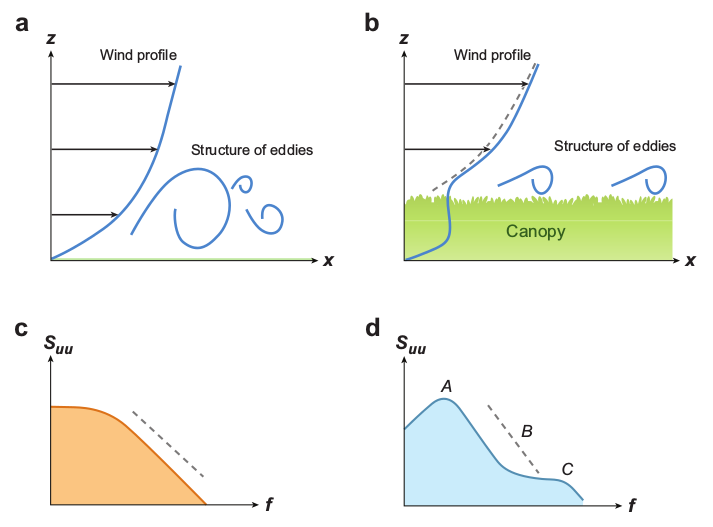
\includegraphics[width=0.7\linewidth]{chapter_1/spectra}
	\caption{Frames \textbf{a} and \textbf{b} show respectively the schematics of the mean flow over a rough wall and a canopy flow; the difference in the eddy size is clear, also the inflection point in the canopy flow velocity profile is obvious.
		Frames \textbf{c} and \textbf{d} show the turbulent spectra for the two different flows above, in the case of rough wall a Kolmogorov type of energy spectrum can be retrieved; in the case of canopy flow it is possible to see  a larger peak in the frequency of the mixing layer instability, a steeper slope in the energy cascade part and high frequency peaks at high frequencies. Image from \citet{de2008effects}.}
		\label{fig:spectra}
	\end{figure}

Is it clear from the literature that the dynamics of the permeable substrate made by vegetation is extremely important and should always be taken into account to fully generalize the physics in such problems involving moving canopies; \citet{nepf2012flow} shows how the interface between aquatic plants and the free flow can be largely modified due to the movement of the fibers (most of the plants arms and branches can be viewed as fibers).

In order to discriminate the different behavior of the fibrous structure it is convenient to introduce some non-dimensional parameters typically used in fluid structure interaction problems:
$$ m^* = \rho_{\beta} / \rho_{\sigma}, \quad C_Y= \rho_{\beta} {U_{\infty}}^2 s^3 / E, \quad s = H/d, $$
where $\rho_{\beta}$ is the fluid phase density, $\rho_{\sigma}$ is the solid phase density, $U_{\infty}$ is a free-stream reference velocity, $E$ is the Young modulus of the solid material, $H$ is a reference length for the extension of the solid structure and $d$ is a reference length for the thickness of the material.
The first parameter is the \textit{mass ratio} ($m^*$), the second is called \textit{Cauchy number} ($C_Y$) and the last one is the \textit{slenderness} ($s$) of the structure.
The mass ratio can be used to quantify the added mass effects caused by solid inertia, however these effects are usually negligible in case of fibrous permeable media.
The Cauchy number defines the static deformation of a fiber caused by the fluid flow; when the Cauchy number is greater than unity, important deformations are expected.
This last parameter is extremely important since it controls a phenomenon called \textit{reconfiguration} that leads to drag reduction (\citet{gosselin2011drag};  \citet{alvarado2017nature}).
The reconfiguration can be defined as the capability of the structure to adopt a new shape when forced by a flow, usually it become more streamlined to reduce its exposed frontal area with the aim to reduce the total drag.
When dealing with this phenomenon one should take into account the frontal area $A$ and the drag coefficient $C_D$ together, in order to avoid misinterpretation of the drag reduction; in figure \ref{fig:cycd} the ratio of the parameter $AC_D$ has been represented for different natural structures against the Cauchy number and it is evident that for a $C_Y>1$ a drastic drag reduction can be observed.

\begin{figure}[h]
	\centering
	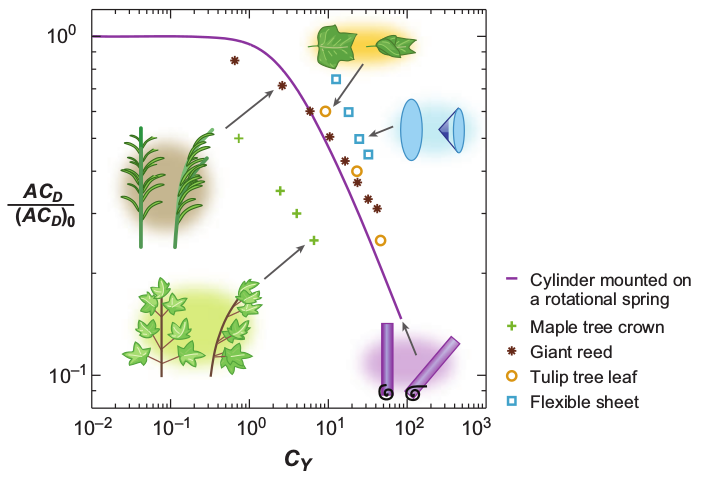
\includegraphics[width=0.7\linewidth]{chapter_1/cy_cd}
	\caption{Effects of the Cauchy number $C_Y$ on drag reduction. The drag reduction is represented as the ratio between the frontal area $A$ and the drag coefficient $C_D$ in dynamic conditions, divided by the same product wider static conditions (subscript). Image from \citet{de2008effects}}
	\label{fig:cycd}
\end{figure}

The overall reconfiguration of the permeable medium can lead to pressure recovery and a wake regularization when applied to a bluff body, as the experiments by \citet{gosselin2011drag} show.

Another important non-dimensional number is the \textit{reduced velocity} ($U_R$), that can be derived from the previous ones:
$$ U_R = \sqrt{C_Y s / m^*}$$
This number is used when dealing with vortex induced vibrations of slender structures; when it is near one, dynamical coupling between the fluid and the structure is expected, such as resonance or lock-in phenomena (self-excited vortex-induced vibrations accompanied by the synchronization of the frequency of vortex formation with the frequency of structure vibration).

Canopies can also help to prevent separation in the presence of adverse pressure gradients. \citet{belcher2012wind} have carried out an analysis of the flow over a hill covered with canopies using numerical and experimental data; the authors show how the permeable layer can present a re-circulation region inside the canopy in the decreasing slope side of the hill. This zone move the separation away from the flow over the hill to the internal structure of the canopy.
%In this sense when we look at the "global" hill (ground and canopy layer) the reversed flow typical of this geometry is not present.

It is important to point out that the above results are restricted to fibrous or slender structures and they cannot be extrapolated in general for different porous structure and shapes, even though similar mechanisms are expected.

The research on canopy flow embraces a wide range of configurations and this makes very difficult the comparison of the results since most of the authors use very different models in various regimes of velocities, using flexible structures with very different shapes.
Even if experiments are easier to find, like \citet{segalini2011experimental}, \citet{segalini2013scaling}, \citet{maza2013coupled}, \citet{barsu2016drag} and \citet{alvarado2017nature}, there is no quantitative mathematical model established for the fluid and structure equations and almost all models available rely on empirical correlations that fit the data in each different application.


\section{Models for flows through porous surfaces}
\label{ch:model_porous}

In this section we want to show some insight of the key characteristics that a model of flows through poroelastic layers should have.
In order to be as clear as possible we have taken as example a very simple geometry to sketch the problem; the flow over a wall that includes multiple flexible filaments (in the hypothesis of highly packed fibers the medium can be treated like a porous medium). 
This simple geometrical configuration still has all the characteristic and difficulties of more interesting applications, such as a bluff body with a poroelastic layer.

\begin{figure}[h]
	\centering
	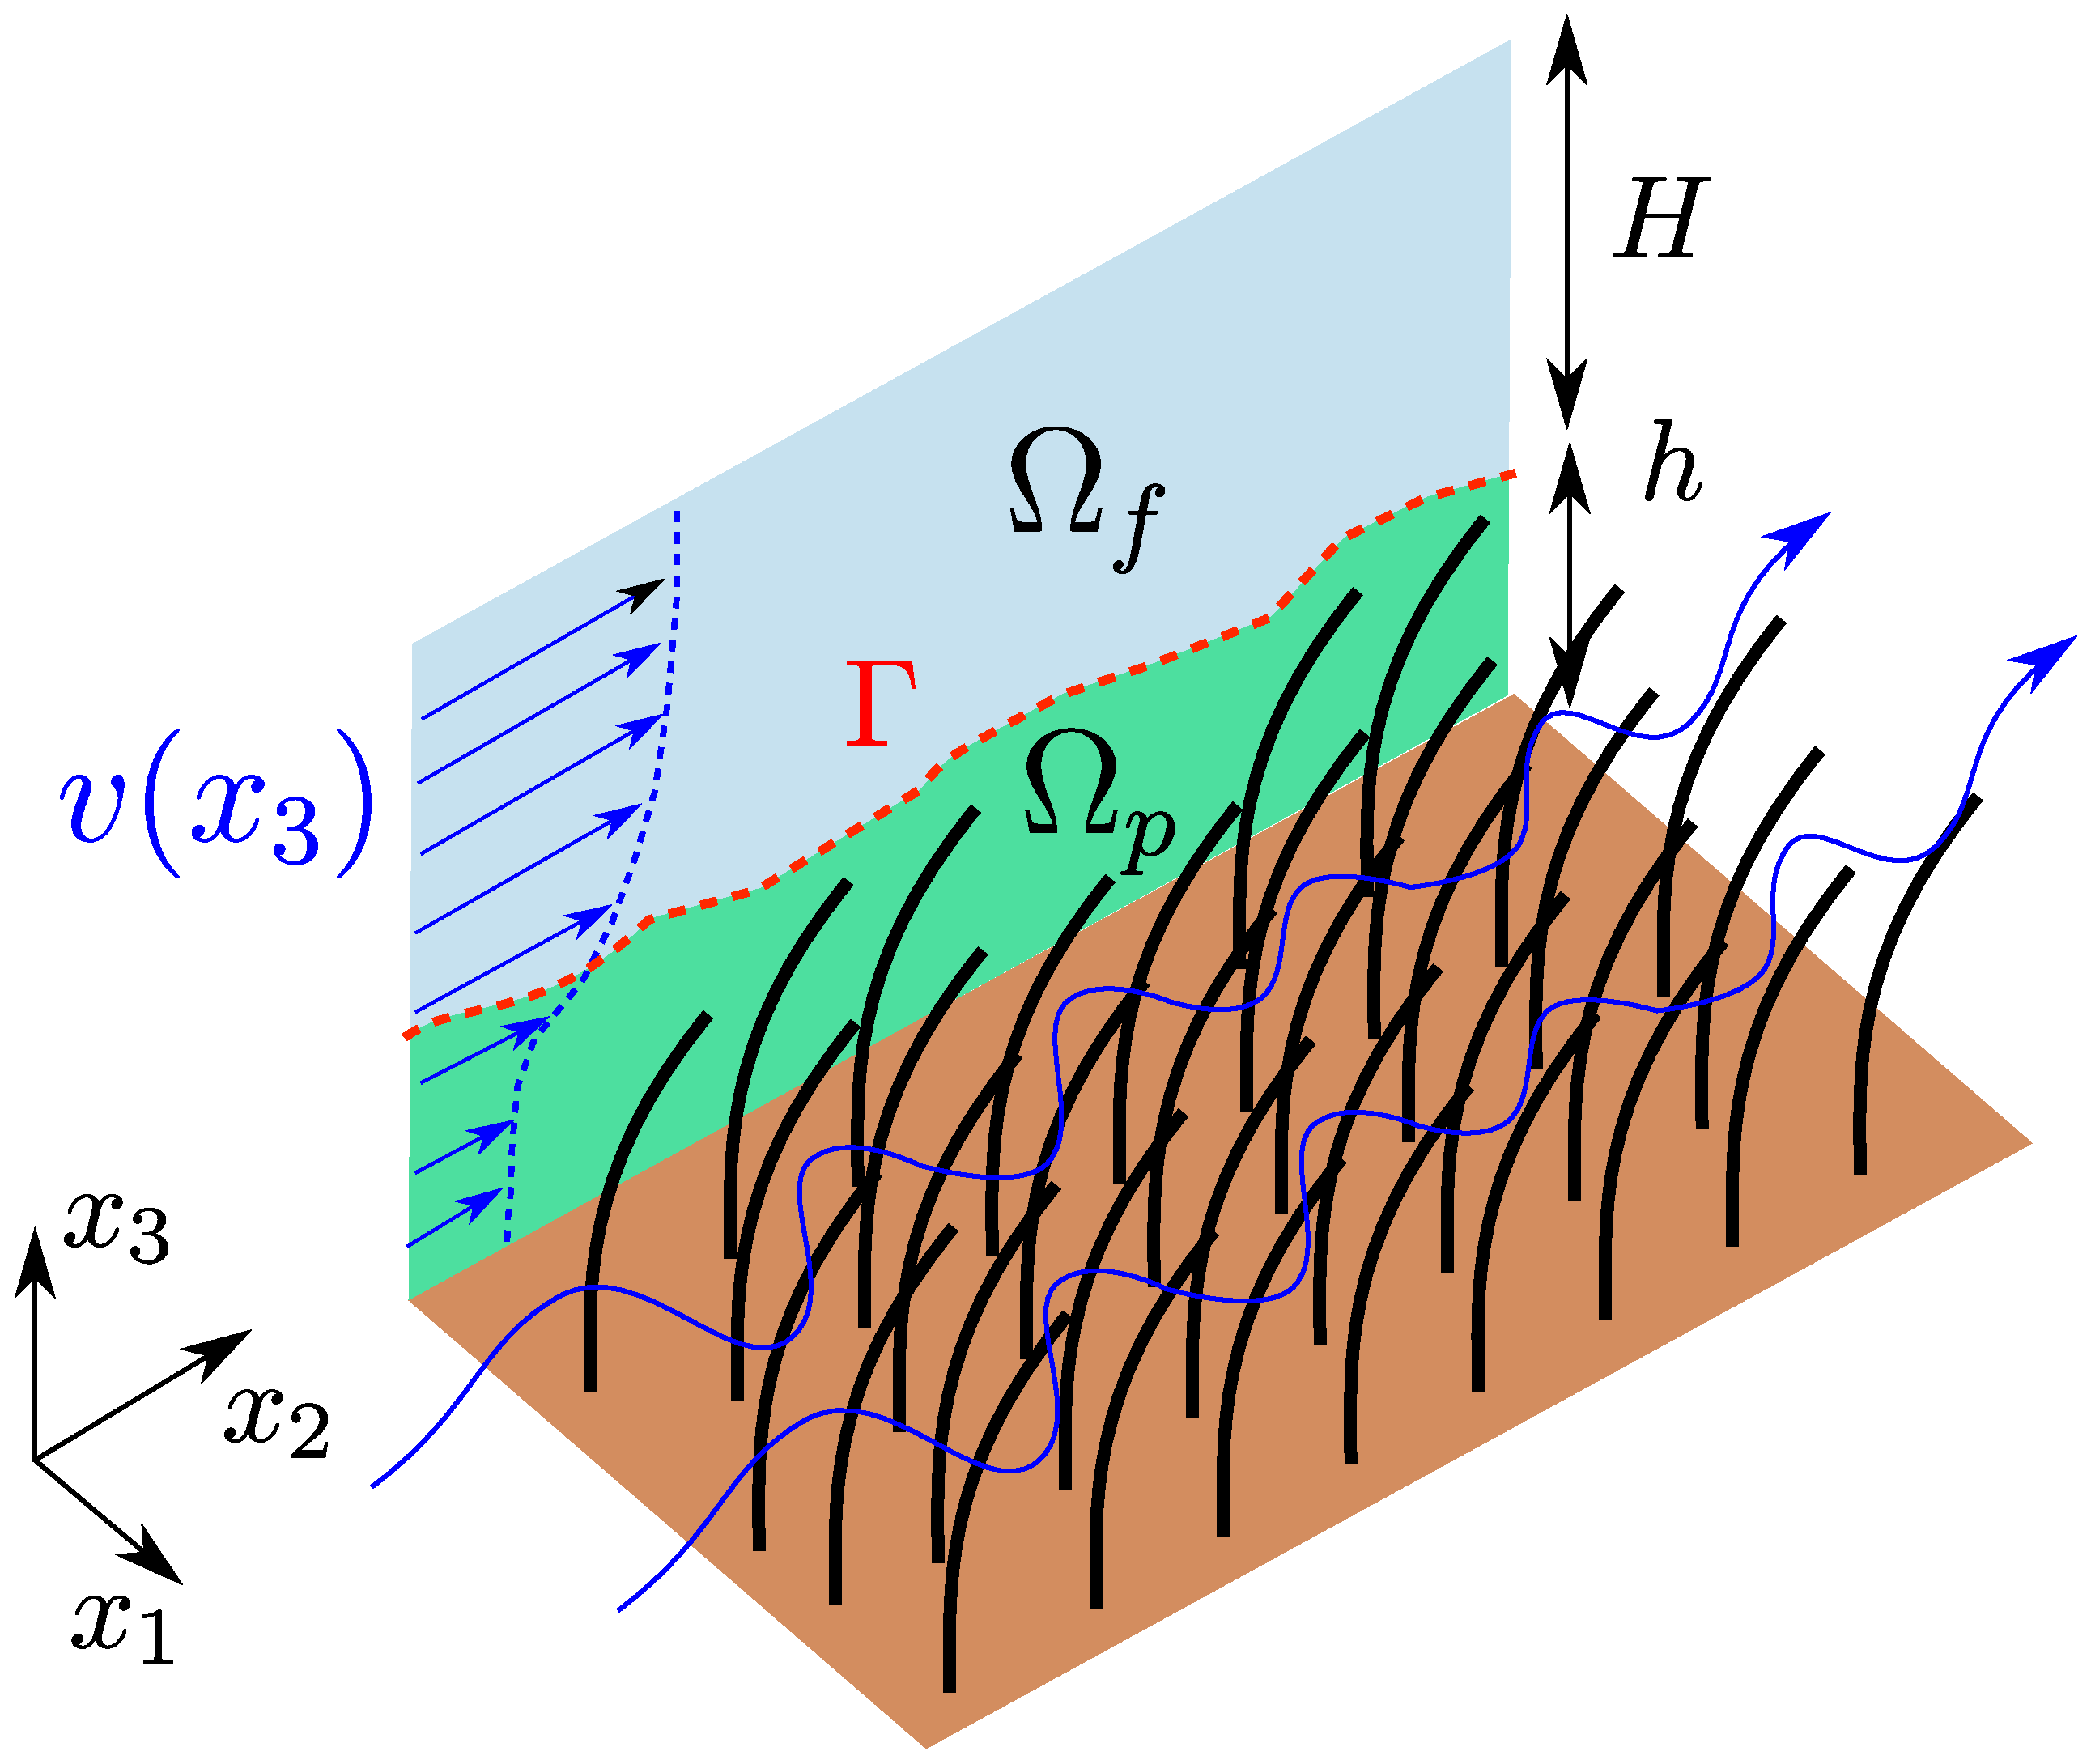
\includegraphics[width=0.7\linewidth]{chapter_1/problem_schema}
	\caption{Sketch of a fully developed flow over a poroelastic surface made of multiple filaments.}
	\label{fig:schema_problem}
\end{figure}

Figure \ref{fig:schema_problem} shows a graphical representation of such a flow; the main fluid direction is aligned with the $x_1$ axis and the projection of the stream-wise component of the velocity is shown in the plane $x_1 - x_3$.
Such flow can bend the filaments that can show a more or less coherent response.
The surface that envelops all the filaments lid ($\Gamma$) defines the limit between the region of free flow ($\Omega_{f}$) and that inside the poroelastic medium ($\Omega_{p}$). Its projection is shown in the  $x_1 - x_3$ plane.

In order to computationally solve this problem there are some key points to address:
\begin{itemize}
	\item Length scales: the flow presents interaction at multiple scales. The flow can develop Kelvin–Helmholtz type instabilities on the interface and they can even penetrate inside the medium and brake up to very small scales eddies. In order to resolve this complex dynamics one should use a very fine numerical mesh (highly computationally expensive) or come up with a model (like in the context of turbulence modeling).
	Turbulence dynamic can be also problematic; the hypothesis that pore size eddies can exist deep inside the porous medium is still object of some debate in the community.
	How to deal with such small scale dynamics and/or find a model is not an easy task. 
	
	\item Compliance (fluid-structure interaction): if the filaments are flexible, they can bend and swing due to the fluid load.
	We have to take into account a structural model for the filaments (by using, for example, the Bernoulli beam equation), including also the computation of energy that the swing motion re-inject inside the fluid.
	This two-way coupling could also be really computational expensive in the presence of a large number of filaments. If the flexibility is important, one should in principle take into account also the contact and repulsion (elastic coupling) between the fibers.
	If the porous medium has more complicated shapes (like the scales in the butterfly wing) to come out with a simplified model for the solid dynamics is even harder and the use of a general finite elements discretization is probably a necessity (increasing also the computational cost of the problem).
	Another approach consists in deriving a "rheological" model for the medium, in which the average mechanical properties can be found.
	Such models are applicable only to porous media where the solid inclusions are connected to each other. Such average methods are convenient computationally but their mathematical description can be difficult.
	
	\item Anisotropy: the model used should be capable to treat permeable surfaces that have different responses when stressed in different directions. For instance, the geometrical arrangement and/or the mechanical properties of the medium can be non-homogeneous, so that the medium can appear more permeable in one direction and show a preferential flow path. The different reaction for a specific direction can be modeled with a tensorial parameter as for the case of the permeability tensor that is basically a generalized drag coefficient.
\end{itemize}

\citet{dupont2010modelling} performed a LES simulation introducing a two-way coupling for the fluid-structure interaction problem over a carpet of fibers. They validated their simulations with video recording of a similar experiment and the frequency measurements of the Kelvin–Helmholtz instabilities at the interface agrees very well.
They have not specified the computational configuration used, but they have mentioned an important high performance computing center in the acknowledgment which made us assume that the computational power involved was substantial.
Recently, also \citet{marjoribanks2017does} have adopted a similar approach.

Some other examples that solve the fully coupled problem directly are discussed by \citet{monti2017large}, \citet{pinelli2017pelskin}, \citet{favier2017pelskin} and \citet{revell2017pelskin}, but in their cases the number of filaments is small and so they can be assimilated to isolated filaments rather than to a poroelastic carpet.

Due to the computationally cost of solving the problem directly, the scientific community has came out with other approaches that treat the porous domain with a generalized model that does not resolve the fine scales inside the medium, but instead expresses them as a function of the length scales present in the fluid domain $\Omega_{f}$.

These are called homogenization approaches and the key points in such methods are:
\begin{itemize}
	\item The division of the overall domain in two different parts: the fluid domain $\Omega_{f}$ and the porous domain $\Omega_{p}$;
	\item Two different fluid models are used in the two domains. In $\Omega_{f}$ the Naver-Stokes equations for incompressible Newtonian fluids are solved. In the porous part there are a number of different models that adds source terms in the former equations to take into account the presence of the porous medium;
	\item The two domains should be coupled together with a boundary condition at the interface or a transitional region around the interface is added with its specific treatment;
	\item A model for the structural mechanics. It can be an averaged model or it can solve the mechanic equations directly.
\end{itemize}

The key points shown above are extensively discussed, in chapter \ref{ch:vans}, for the homogenization method chosen in this thesis.
However, in the next section the two main branches in literature, that take into account the presence of a porous medium layer are summarized in order to give a panoramic on the possible choices.


\subsection{Isotropic drag models}
\label{sec:canopy_eq}

In the case of flow through vegetation (canopy flows) it is common to use an isotropic drag model\footnote{the drag is equal along the three principal directions of the medium.} to parameterize the drag of the canopy.
The drag can be a function of the wall normal direction, but in most of the applications it is taken as a constant.
The isotropic hypothesis can be correct in case of dense vegetation, even if the normal component of the resistance should be smaller.
However the resistance in the vertical direction can be approximated in this manner in channel flows where the mean flow is mostly streamwise. On the contrary, in applications where the transpiration at the interface is important (wake control of bluff body) the isotropic drag model is, certainly, not the most adequate.

The drag resistance is included in the Navier-Stokes equations as a source term:

\begin{equation}
\derp{\vb}{t} + \vb \cdot \nabla \vb = -\frac{1}{\rho_{\beta}} \nabla \pb + \nub \nabla^2 \vb - \dfrac{1}{2} C_D a |\vb| \vb, 
\label{eq:mom_cd}
\end{equation}

where the subscript $\beta$ indicates variables defined in the fluid phase, and $C_D$ the drag coefficient of the isolated fiber.
The parameter $a$ is the frontal area per unit volume of the vegetation, and it is function of the porosity of the medium.
The drag term is quadratic in the velocity, but there is some evidence in the literature that the reconfiguration phenomenon can change this relationship (\citet{gosselin2011drag}; \citet{alvarado2017nature}).

From our point of view this approach lacks of strong mathematical formalism. As a matter of fact the definition of the additional terms of the equations heavily relies on empirical relations.
Another issue is that the isotropic hypothesis rules out the possibility to model the anisotropic nature of most surfaces in which we are interested. %\footnote{as equation \eqref{eq:max_dr} suggests, the difference in the permeability along each direction can be important for drag reduction.}.

In the field of flows through vegetation some authors have successfully used this approach, for example \citet{maza2013coupled} and \citet{maza2015tsunami} used it to study wave attenuation and \citet{ghisalberti2004limited}, \citet{battiato2014single} developed simple models for the 2D mean flow over a canopy.


\subsection{Homogenization models}

In this section we want to introduce the most used approach to derive the equations valid in the porous domain.
The fundamental idea is to build a micro-scale model, for both the fluid and the solid, and then derive the macro-scale equations using some averaging operator over the micro-scale.

The two most used homogenization methods are the \textit{Volume Averaging} method (\citet{whitaker2013method}) and the \textit{Multiple Scales} method (\citet{mei2010homogenization}) which can be broadly classified as perturbations methods. 
The key differences and the main results retrieved using these approaches are presented in the following.


\subsubsection{Volume Averaging}
\label{sec:vans}

The method of Volume Averaging has been developed to treat transport equations in porous media applications; in this case the presence of two different length scales is obvious, as it can be evinced from figure \ref{fig:porsystem}.
	
	\begin{figure}[h]
		\centering
		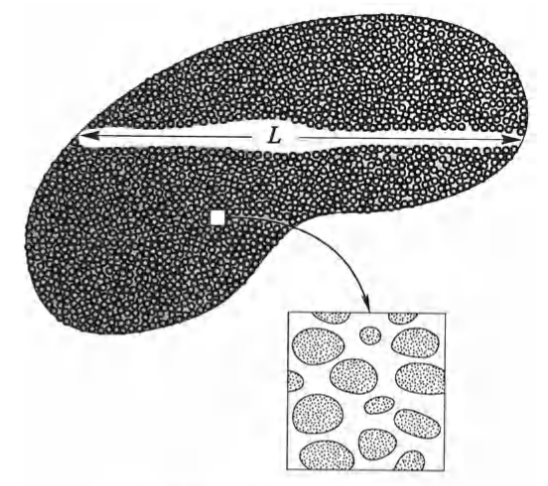
\includegraphics[width=0.5\linewidth]{chapter_1/por_system}
		\caption{Schematics of a porous medium of size $L$, with a zoom on the microscopic structure and its scale $\ell$. Image from \citet{whitaker2013method}.}
		\label{fig:porsystem}
	\end{figure}

The core idea of the methods is to firstly define an average operator as $$\meani{\psi} = \dfrac{1}{\volb} \displaystyle\int_{V} \psi \, dV$$ in this case the variable $\psi$ represents any vector or scalar variable in the system of equations that we want to homogenize; for Navier-Stokes equation $\psi$ is the velocity and the pressure. In the above operator $\volb$ is the fluid fraction present inside a reference volume $V$.

The average operator has the purpose to homogenize the equations. The second crucial step of the method is to decompose the variables as proposed by \citet{gray1975derivation}:

\begin{equation}
\psi =   \underbrace{ \meani{\psi} }_\text{O($L$)}  +  \underbrace{\tilde{\psi} }_\text{O($\ell$)}
\label{eq:vans_decomp}
\end{equation}

\noindent Equation \eqref{eq:vans_decomp} shows how each variable can be decomposed into an averaged part which contains only spatial variations at the macro-scale $L$ and a \textit{fluctuation} part that contains only the micro-scale $\ell$ spatial variations.

Also the decomposition can be substituted in the transport equations that we want to average, and after some mathematical manipulations it is possible to retrieve the new averaged equations that include only variables of order $L$.
Since this is the method chosen to develop our work, all the technical details are explained in chapter \ref{ch:vans}.

To introduce briefly some other aspects about this method, we show, as an example, how to derive the homogenized version of the Stokes equation. The described problem is a steady flow inside a rigid porous medium, like the one in figure \ref{fig:porsystem}.
The Stokes equation valid for the fluid phase, indicated with the $\beta$ subscript, reads:

\begin{equation}
0 = - \nabla \pb +\mub \nabla^2 \vb,
\label{eq:stokes}
\end{equation} 

It is important to specify that equation \eqref{eq:stokes} is valid only in the fluid phase and in order to solve it we have to consider a no-slip boundary condition at the interface with the solid phase, with the difficulties that come to define the complex structure of the solid inclusion.
Applying the Averaging Method, we can derive a homogeneous version of \eqref{eq:stokes} that is valid in all the domain that includes the two different phases, the solid and the liquid one.
The homogenized version of \eqref{eq:stokes} is the well known Darcy's equation:
$$\vbmi = -\dfrac{ \mathbf{K} }{\varepsilon \mub} \nabla \pbmi,$$
developed with this approach by  \citet{whitaker1986flow}.

The Darcy's equation allows to recognize two additional quantities that arise from the averaging procedure, the first one is a scalar called porosity $\varepsilon$ that represents the ratio between the volume of the fluid inside a reference volume over the total volume.
The second one is the tensor $\mathbf{K}$ called permeability tensor and it expresses the resistance of the porous medium that affects the flow in its motion.
The term $\mathbf{K}$ plays the same role as $C_D a$ in the isotropic drag model; the main difference is that the permeability tensor can be computed directly from the geometry of the medium (see chapter \ref{ch:vans}), i.e. it does not rely on empirical relations.
In addition, the tensorial nature of this terms allows us to model porous inclusions that are anisotropic.

Applications of the theory include flow where inertial terms are not negligible (\citet{whitaker1996forchheimer}), porous media with small deformations (\citet{whitaker1986flow2}) and with high deformations (\citet{hussong2011continuum}), turbulent problems (\citet{soulaine2014}, \citet{breugem2006influence}), interface between a permeable medium and a free flow (\citet{beaver}), multi-phase systems (\citet{whitaker1973transport}), heat transfer (\citet{carbonell1984heat}) and sound propagation (\citet{firdaouss1998some}, \citet{lafarge1998sound}).

It is impossible to go into details in the derivation of the equations for each specific problem, but the key point here has been to show the differences between this method and the isotropic drag model of the previous section.

\subsubsection{Multiple Scales}

The multiple scales method presents analogies to the previous one and it has also been applied to similar problems in the context of porous media applications.

In this method we start with the assumption of scale separation between $\ell$, the micro-scale, and $L$, the macro-scale.
The scale separation factor can be defined as $\epsilon = \ell/L \ll 1$.
Using the same examples as the previous section, we show how to compute the homogenized version of the Stokes equation for fluid flow through porous media.
We introduce the micro-scale and the macro-scale coordinates defined respectively as:
$$
 X_i = \dfrac{\tilde{x}_i}{L}, \quad   x_i = \dfrac{\tilde{x}_i}{\ell},
$$
where $x_i$ are the original eulerian coordinate of the problem.
Using the above separation factor it is possible to expand the pressure and velocity as:
$$
\psi(X_i, x_i) = \psi^{(0)}(X_i, x_i)  +\epsilon \psi^{(1)}(X_i, x_i) +\epsilon^2 \psi^{(2)}(X_i, x_i) +O(\epsilon^3),
$$

Substituting this decomposition inside the equation \eqref{eq:stokes} it is possible to derive a set of hierarchical equations, one for each order of the expansion.
It can be shown that analyzing each equation in the set the homogenized equation yields:

\begin{equation}
{v_i}^{(0)} = -K_{ij} \dfrac{\partial p^{(0)}}{\partial X_j},
\label{eq:darcy_ms}
\end{equation} 

In which either the pressure or the velocity fields appears only at the order zero, and the equation depends only on the macro-scale length.

The same permeability tensor $\mathbf{K}$ as before is found, with the same definition and interpretation.
It is clear that for this simple problem we end up with the same homogenized equation; the point that has changed is the starting hypotheses of the method and the mathematical development.

A full analysis of the dualism of the two approaches can be found in the work by \citet{davit2013homogenization}.

The multiple scales method has also been used to study many other problems: inertial effects (\citet{mei1991effect}, \citet{skjetne1999new}), coupling between a free fluid and a porous media (\citet{mikelic2000interface}), porous media with small deformations (\citet{auriault1977etude}), heat conduction in composites (\citet{auriault1983effective}), rigid and moving permeable layers (\citet{zampogna2016fluid}, \citet{ugis} and \citet{zampogna2017pelskin}).

%There is also another homogenization based method called \textit{Mixture Theory} that is also worth a mention.
%It is based on a similar approach as the previous ones and \citet{rajagopal2007hierarchy} showed that it is possible to retrieve the same equation as the previous two methods in case of porous media flow.


\section{Stability of flows over permeable surfaces}
\label{sec:stability}

Flows through submerged aquatic plants exhibit large scale vortices at the top of the vegetation,
advected along the flow direction and causing a periodic waving of the plants, referred to as
monami (if the fluid is air) and honami (in case of water) (\citet{inoue1955studies}, \citet{ackerman1993reduced}).
The effect of the onset of the monami is depicted qualitatively in figure \ref{fig:monai_evol}.

\begin{figure}[h]
	\centering
	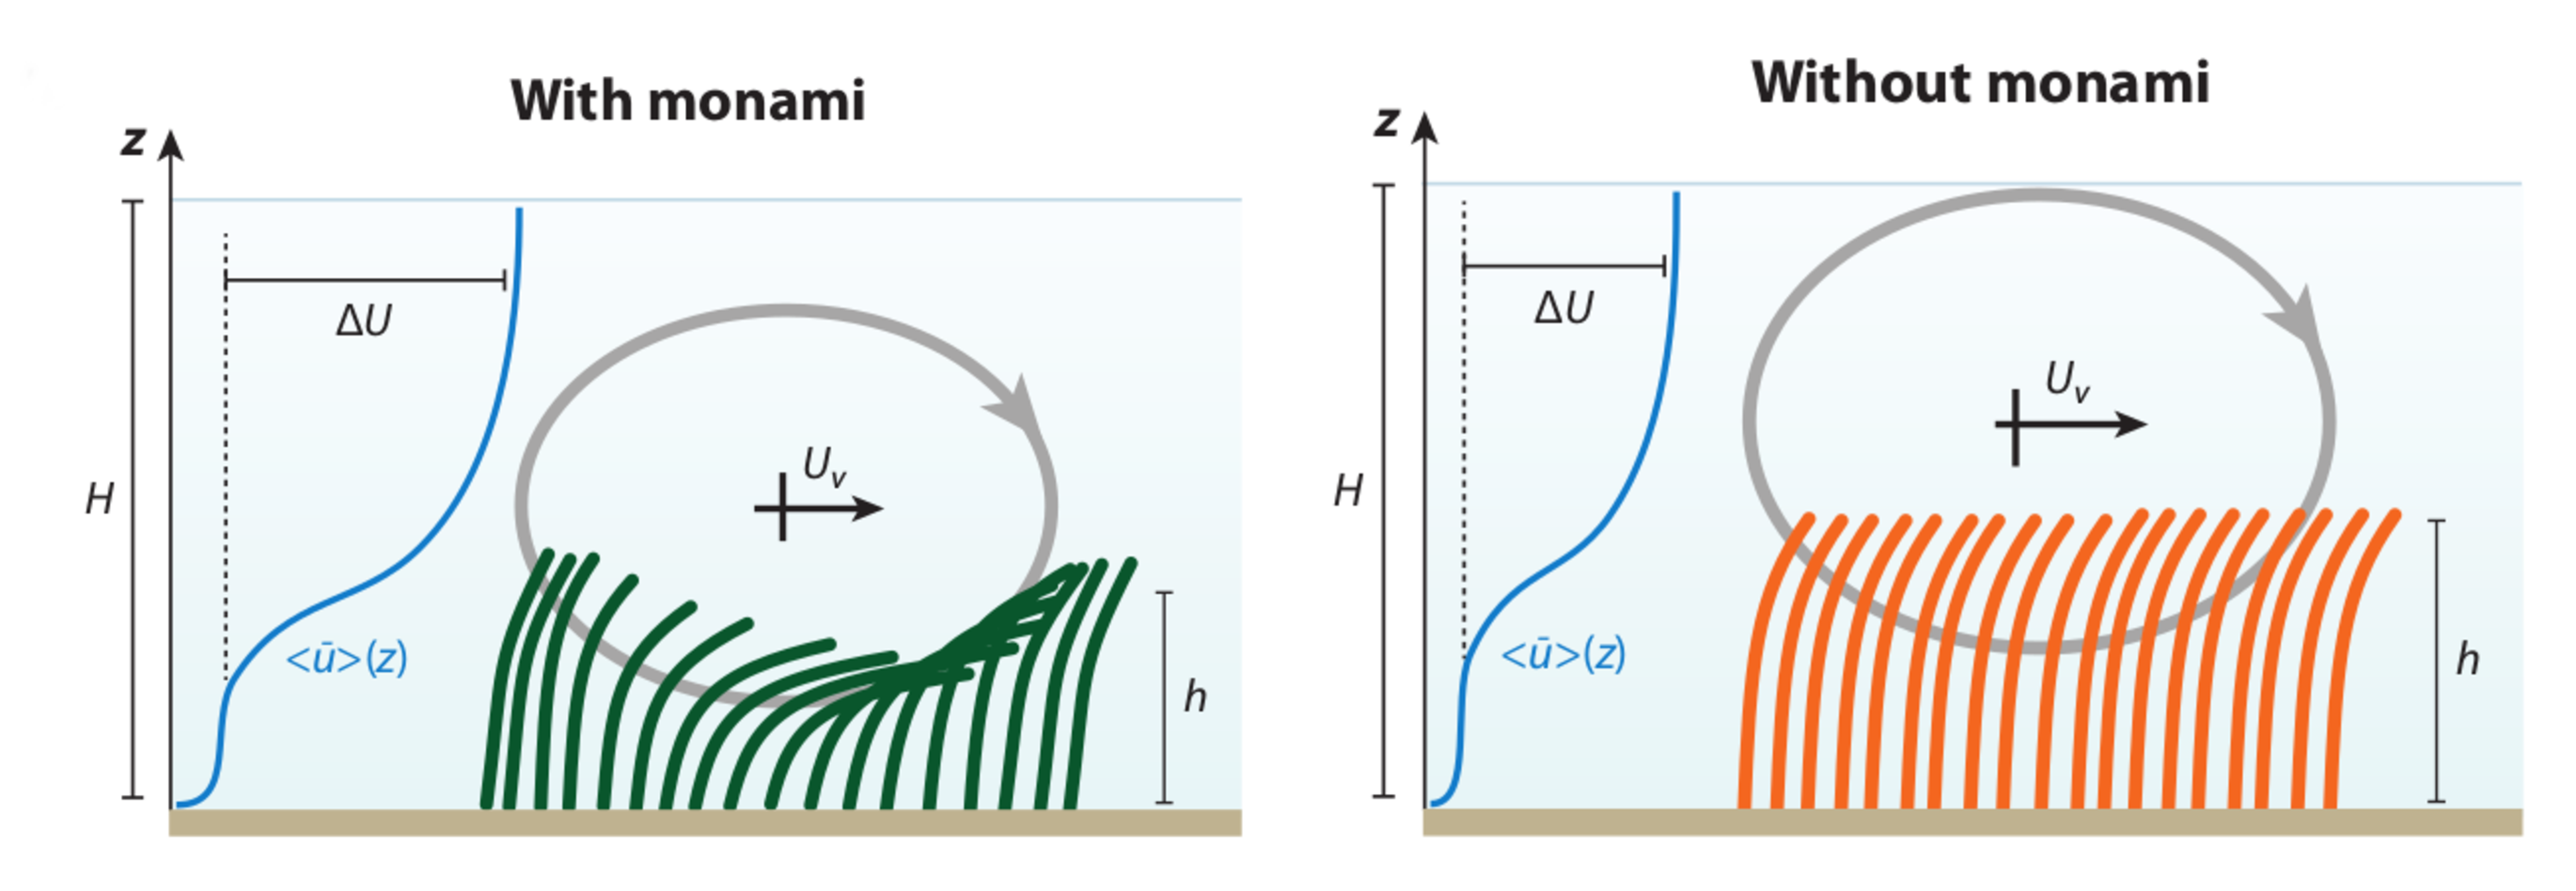
\includegraphics[width=1\linewidth]{chapter_1/monami}
	\caption{Left: when the drag of the canopy is large enough it generates canopy-scale vortices by Kelvin-Helmholtz instability. These vortices may interact with the flexible vegetation and generate a waving motion called monami. Right: when this interaction is too weak, the canopy only bend. Image from \citet{nepf2012flow}.}
	\label{fig:monami}
\end{figure}

Vortices arise from the nonlinear amplification of a Kelvin-Helmholtz instability mode, related to the presence of an inflection point in the base flow profile (\citet{asaeda2005morphological}); the profile itself is inflectional because the fluid is slowed down by the drag exerted by the canopy, whose modeling has recently been addressed (\citet{py2004mixing}; \citet{singh2016linear};  \citet{zampogna2016instability}; \citet{tilton2008linear}).
The correct prediction of the onset and characteristics of the Kelvin-Helmholtz instability is important to assess the effects of turbulence (\citet{finnigan2000turbulence}, \citet{jimenez2001turbulent}) in particular to:

\begin{itemize}
	\item understand how the vertical exchange of momentum occurs (\citet{ikeda1996three}).
	\item clarify how the transport of $\text{CO}_2$ and dissolved nutrients or sediments take place. This exchange occur between the
	obstructed vegetation flow and the free overflow motion (\citet{gambi1990flume}, \citet{eckman1987role}, \citet{grizzle1996hydrodynamically}).
	\item assess the changes in the morphology of the vegetation in inland or coastal wetlands in
	response to continuous periodic forcing (\citet{asaeda2005morphological}, \citet{patil2010characteristics}).
\end{itemize}

One of the possible approaches to study how and when these instabilities start is the linear stability analysis. In the following section we briefly introduce the key assumption and simplifications of the method, and in the next section some results in the context of permeable surfaces are presented.


\subsection{Stability theory generalities}

Stability theory covers the modeling of transition of fluid systems towards unstable states eventually leading to turbulence.
The theory gives us a fast and robust method to compute the frequency and grow rate of the unstable mode, if there is any, in the base flow.

The linear stability relies on the decomposition of the flow variables $\mathbf{q}$ into a steady-state part $\overline{\mathbf{q}}$, called base flow, and an unsteady part $\widetilde{\mathbf{q}}$:

$$ \mathbf{q} (\mathbf{x},t)= \overline{\mathbf{q}} (\mathbf{x}) + \widetilde{\mathbf{q}} (\mathbf{x},t) $$
Where the unsteady part is small compared to the steady one. We also simplify $\widetilde{\mathbf{q}}$ with the hypothesis to have a general wave form:
$$  \widetilde{\mathbf{q}} =  \widehat{\mathbf{q}}(\mathbf{x}) e^{i\Theta(\mathbf{x},t)} $$
where $\widehat{\mathbf{q}}$ is the amplitude function and $\Theta$ is the phase of the perturbation.
The choice made to determine the time and space dependency of either the phase function and the amplitude determine a certain hierarchy inside the stability theories. This hierarchy depend on how many directions we consider to be periodic in the amplitude function\footnote{The hierarchy goes from local approach with 2 direction periodic out of 3, to tri-global with all the 3 directions considered space dependent.}.
Figure \ref{fig:table} below present each possible choice in literature and the theory that derives from it.

\begin{figure}[h]
	\centering
	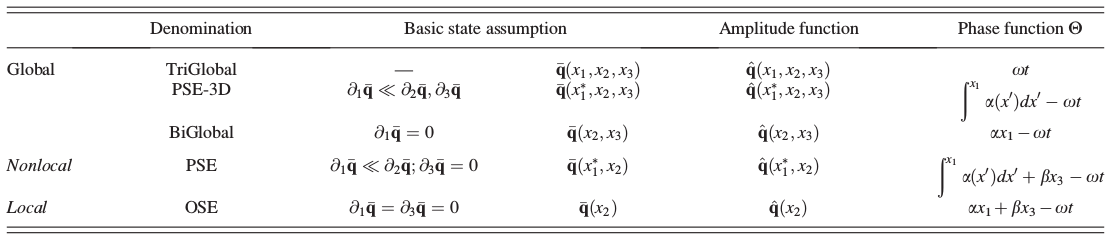
\includegraphics[width=1\linewidth]{chapter_1/table}
	\caption{Classification of modal linear stability theories. Table from \citet{juniper2014modal}.}
	\label{fig:table}
\end{figure}
 
In our case we have limited our study to a local approach build on mode decomposition, \textit{local stability theory} (LST, also known as \textit{ordinary stability equations} OSE in the denomination of figure \ref{fig:table}).
In the LST we make the hypothesis that the amplitude and the base flow depend only on the wall normal spatial coordinate (parallel flow) and the phase function takes into account the periodicity in time and in the streamwise and cross-flow directions.
The last hypothesis should not only be seen as a simplification since there are some problems (such as canopy flows) in which two of the three directions are really homogeneous.
The complete formulation is in the following equation:
 $$  \widetilde{\mathbf{q}}(\mathbf{x},t) =  \widehat{\mathbf{q}}(x_2) e^{i(\alpha x_1 + \beta x_3 - \omega t)}  $$ 
where $x_2$ is the wall normal direction, $\alpha$ is the streamwise ($x_1$) wavenumber, $\beta$ is the crossflow ($x_3$) wavenumber and $\omega$ is the temporal frequency.

Casting this form for the pressure and velocity inside the Navier-Stokes equation, the equations that we get describe the evolution of the perturbations, taking the base flow as an input of the problem.
In order to study the stability of the perturbations in their time evolution, problem known as \textit{temporal stability}, we fix the space perturbation form imposing $\alpha$ and $\beta$ as real numbers (inputs of the problem) and solving for $\omega$ as a complex number.
With such choices the problem became a generalized eigenvalue problem for $\omega$:
$$ A \widehat{\mathbf{q}} =  \omega B\widehat{\mathbf{q}} $$
The solution gives the frequency (real part of the eigenvalues) and the growth-rate (imaginary part) of the perturbation modes (eigenvectors) of the flow.

The above introduction of the method is quite condensed, however there is much literature on the subject (\citet{juniper2014modal}, \citet{criminale2003theory}, \citet{schmid2012stability} and \citet{ortiz2002spatial}). The problem has also been extensively studied in its computational aspects by \citet{canuto1988spectral}.

\subsection{Monami/Honami and Kelvin-Helmholtz rolls}

We have already highlighted that the above framework concerning the stability problem has been applied in some porous media flow (canopy) configurations, also including the vegetation movement.
Because of the flexibility of the vegetation, some theoretical studies have focused on the
modeling of the stems of the aquatic plants and their displacement in response to the forcing by the
water flow (\citet{py2004mixing}; \citet{patil2010characteristics}; \citet{gosselin2009destabilising}; \citet{py2006frequency}).

It has been studied in \citet{finnigan2000turbulence} that these large coherent structures control turbulence dynamics over the canopy. 
Movements of the latter generate sweeps (and ejections) of fluids that generates the counter-rotating stream-wise eddy evolving as Kelvin-Helmholtz rolls.
The complex evolution of vortices is shown in figure \ref{fig:monai_evol}.

\begin{figure}[h]
	\centering
	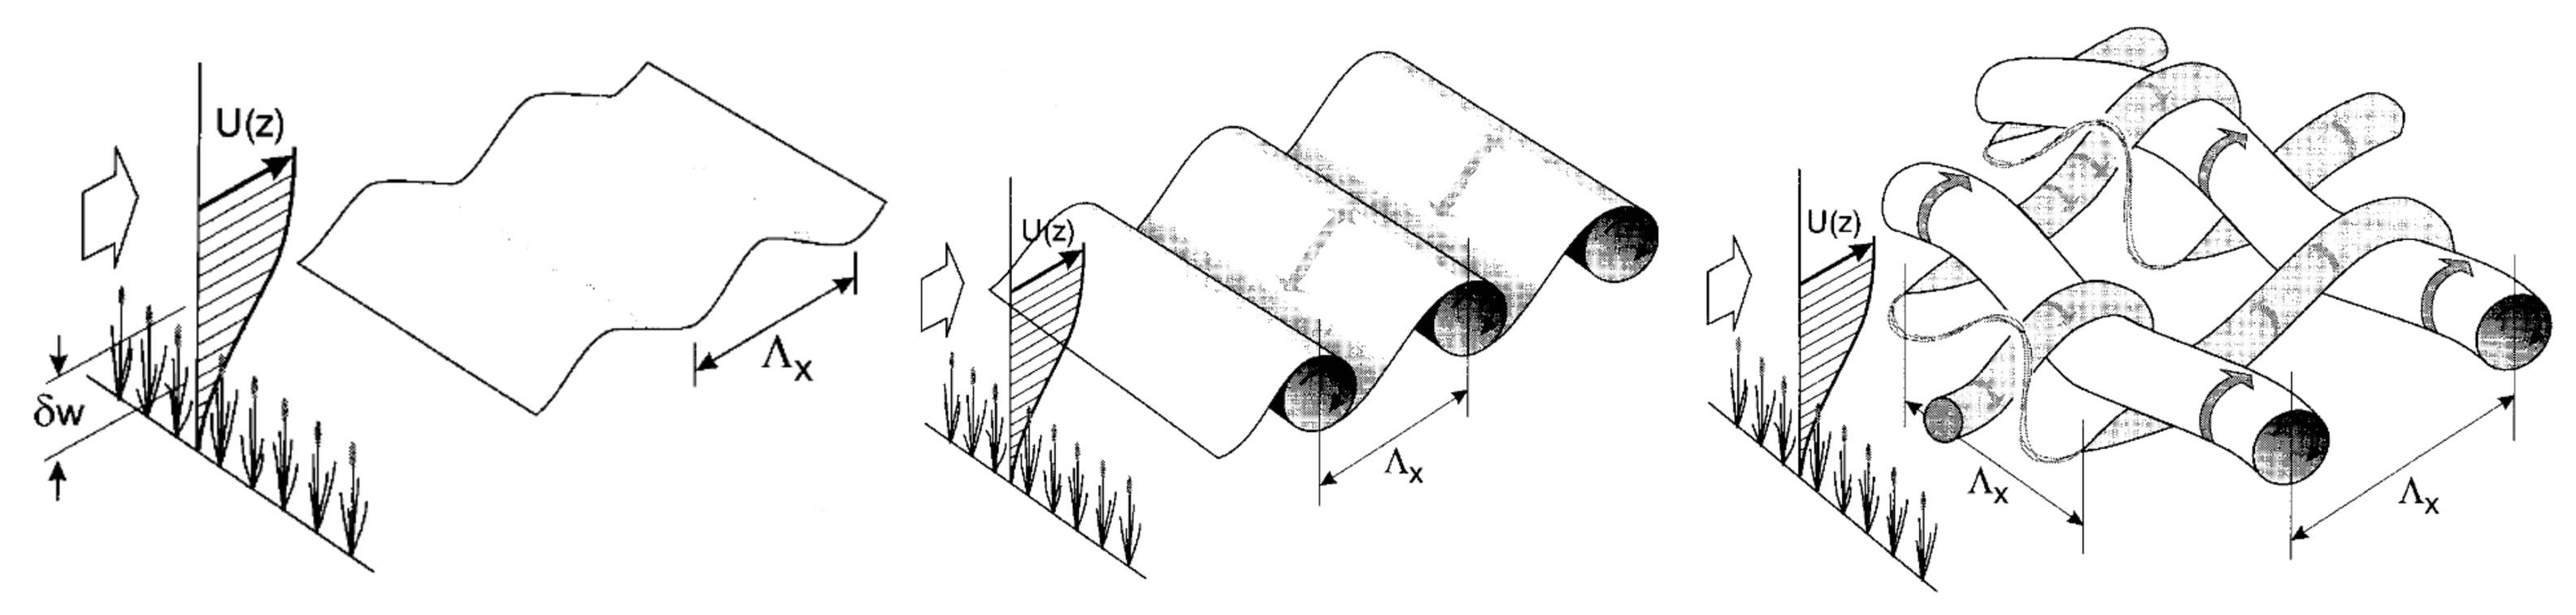
\includegraphics[width=1\linewidth]{chapter_1/finn}
	\caption{Left: first emergence of the Kelvin-Helmholtz instability. The growth-rate is proportional to the shear magnitude at the inflection point. Center: the instability evolves in rollers consisting of high vorticity that are spaced with a similar wave-length $\Lambda_x$ as the previous stage.  Right: secondary instabilities in the rollers lead to their kinking and pairing, coherent structures appear in the transverse and streamwise dimensions. Image from \citet{finnigan2000turbulence}.}
	\label{fig:monai_evol}
\end{figure}


However, Kelvin-Helmholtz vortices occur whether the plants bend or not, and to ascertain causes and effects to first order it is acceptable to focus on rigid porous structures.
The flow over and through a submerged array of rigid, cylindrical pillars has been the basis of the approach of \citet{ghisalberti2002mixing} \cite{ghisalberti2004limited} \cite{ghisalberti2005mass}, who have conducted a series of careful experiments. Their results have often been used by fluid dynamicists to put forth and test theoretical hypotheses to predict the frequency and wavelength of the large scale vortical motion, for a variety of conditions.
The configuration studied consists of a regular grid of rigid pillars, orthogonal to the surface, of identical height $h$.
In some of the theoretical models proposed to analyze the stability of this system, the Rayleigh equation is
used throughout the water channel, with or without a drag term in correspondence of the canopy (\citet{raupach1996coherent}; \citet{py2004mixing}; \citet{singh2016linear}; \citet{zampogna2016instability}; \citet{luminari2016drag}). The same authors have recently demonstrated that the addition of a drag term through the vegetation reduces the amplification factor of the Kelvin-Helmholtz instability throughout the whole range of wave-numbers and increases mildly the wavelength of the fastest growing mode (\citet{zampogna2016instability}; \citet{luminari2016drag}).
In chapter \ref{ch:stability} we study how the perturbation of the base flow affects the predicted amplification factor and wavelength. We also test the difference between the isotropic drag model and the tensorial approach, in order to show which approach is more robust for stability computations.


\section{Conclusions}
The key points of this introductory chapter were to first present the context of this research. We have started explaining that the idea of using porous surface as aerodynamical performance enhancement from various examples in Nature.
Many models based on this idea already exist and we gave an extensive summary of the results present in the literature. We have also presented the key points of the mathematical methods used to derive the porous medium equations that supply a basis for the next chapter in which the volume average method is formally explained.
%Some of the results and the context of the chapter \ref{ch:stability} has been also presented to clarify the connection between the stability analysis and the porous flows.